\chapter{HGP-Clusterer en pratique}
\label{chap:conclusion_partie_II}

%\rouge{25 avril - 1er mai}

Ce chapitre achève la deuxième partie consacrée à la généralisation du Single-Linkage dans l'espace euclidien, avec un certain nombre de considérations où la pratique diffère de la pure théorie.

Premier problème rencontré en pratique (\S~\ref{sec:chapV_partition_stricte}) : il est parfois nécessaire d'avoir une partition stricte des données $\mathcal X$ (et non un recouvrement comme les $K$-polyèdres produits par HGP-Clusterer $\theta^{\mathrm{HGP}}$).

Nous décrivons ensuite (\S~\ref{sec:chapV_k2_empirique}) la mise en œuvre optimisée pour $K=2$ ne nécessitant que le calcul de la triangulation de \textsc{Delaunay} standard et qui nous a permis d'obtenir des résultats empiriques à la fois sur des données synthétiques 2D et des données réelles 8D (les huiles d'olive italiennes) pour illustrer la supériorité de HGP-Clusterer face à HDBSCAN \cite{BibiAppliedNetworkScience}. 

Il arrive aussi parfois que les données $\mathcal X$ soient de trop grande dimension pour pouvoir calculer la triangulation de \textsc{Delaunay} (phénomène dit du «~fléau de la dimension~», \emph{curse of dimensionality} \cite{Pestov2000CurseDimensionality} en anglais). Ou bien les données peuvent tout simplement ne pas provenir de l'espace euclidien. (Supposons qu'on ait une matrice de distance, éventuellement creuse, représentant des données dans un espace métrique quelconque.) En ce cas, nous pouvons recourir à un autre complexe que celui de \v Cech : le complexe de \textsc{Vietoris--Rips} (\S~\ref{sec:chapV_vietoris_rips}).

Pour terminer ce chapitre, nous revenons en \S~\ref{sec:chapV_reduction_dimension} sur l'objet mathématique au cœur de HGP-Clusterer, et qui contient toute l'information de la hiérarchie $K$-NN : la mosaïque de \nom{Delaunay} d'ordre $K$.
Nous l'avons utilisée à des fins de clustering, alors nous avons montré qu'il suffisait d'extraire un arbre minimum couvrant sur certaines de ses cellules. Mais on aurait pu l'utiliser pour d'autres fins de structuration automatique de données !
Nous esquissons une direction de travail encore ouverte : utiliser la mosaïque comme support d'une réduction de dimension de type UMAP, mais en recourant à des interactions d'ordre supérieur.

%\Contributions{}

\section{Et lorsqu'on impose une partition stricte des données ?}
\label{sec:chapV_partition_stricte}

Jusqu'ici, HGP-Clusterer a été présenté comme une hiérarchie exacte de $K$-polyèdres. Ce point est fondamental : pour $K\ge2$, l'objet naturel n'est pas une partition de $\X$, mais un recouvrement de $\mathcal X$ (ou bien une partition des $(K-1)$-simplexes). 

Un point peut appartenir à plusieurs $K$-polyèdres, parce qu'il peut apparaître dans plusieurs $(K-1)$-simplexes situés dans des composantes différentes du graphe $\Gamma_K(\mathcal X)_r$ ; c'est précisément l'information géométrique portée par les intersections d'ordre supérieur.

En revanche, la plupart des bibliothèques de clustering, des métriques usuelles, des tableaux de résultats et surtout des problèmes concrets posés à la fois par les mondes académique \& industriel veulent une assignation unique d'un cluster à chaque point. 
% Il faut donc distinguer nettement deux opérations :
% \begin{enumerate}
%     \item construire la hiérarchie exacte des $K$-polyèdres ;
%     \item extraire, seulement à la fin, une partition stricte compatible avec cette hiérarchie.
% \end{enumerate}
Il va nous falloir ``réparer'' cela. Pour ce faire, nous proposons un post-traitement qui conserve telle quelle la première étape de la construction de la hiérarchie des $K$-polyèdres.

Soit $\mathcal F_K$ l'ensemble des $(K-1)$-simplexes effectivement construits par l'algorithme (ce sont les sommets du graphe dual utilisé par HGP-Clusterer ; dans la version standard de l'algorithme, $\mathcal F_K$ correspond aux simplexes de \textsc{Gabriel}). 
Après traitement de cette hiérarchie (\emph{exempli gratia}, condensation de l'arbre et sélection des clusters pertinents par excès de masse comme HDBSCAN \cite{HDBSCAN2017} le fait), chaque face $\tau\in\mathcal F_K$ reçoit soit une étiquette de cluster
\[
    \ell(\tau)\in \{0,\ldots, q_\mathrm{clust}-1\},
\]
soit l'étiquette $-1$ si la face n'appartient à aucun cluster sélectionné (considérée comme du bruit).

L'implémentation associe à chaque face $\tau\in\mathcal F_K$ un score local positif. Dans la version par défaut, ce score est
\[
    S_\tau
    \eqdef
    \sum_{\substack{\sigma\supset\tau\\ |\sigma|=K+1}}
        \psi\bigl(\rho(\sigma)\bigr),
    \qquad
    \psi(t)=\frac{1}{t^p},
\]
où $\rho(\sigma)$ désigne le rayon de naissance du $K$-simplexe $\sigma$ dans la filtration. Plus généralement, $\psi$ peut être remplacée par toute fonction de poids décroissante. Le choix uniforme $\psi\equiv1$ est possible, mais le choix $1/t^p$ reflète plus exactement la densité locale, qui est au cœur du modèle mathématique derrière HGP-Clusterer.

Pour éviter qu'un point incident à beaucoup de faces soit artificiellement surpondéré, chaque point $x\in\X$ normalise la masse de ses faces incidentes par
\[
    T_x
    \eqdef
    \sum_{\substack{\tau\in\mathcal F_K\\ x\in\tau}} S_\tau.
\]
La masse d'une face dans l'arbre condensé est alors
\[
    m_\tau
    \eqdef
    S_\tau
    \sum_{x\in\tau}\frac1{T_x},
\]
avec la convention $1/T_x=0$ lorsque $T_x=0$. Ainsi, lorsqu'un point appartient à au moins une face, il distribue une masse totale égale à $1$ entre les faces qui le contiennent. C'est ce poids $m_\tau$, et non le simple comptage des faces, qui est utilisé par le seuil \texttt{min\_cluster\_size} dans l'arbre condensé (même idées algorithmiques que HDBSCAN).

La conversion en partition stricte se fait ensuite par vote pondéré. Pour tout point $x\in\X$ et tout cluster $c$, on définit
\[
    V_x(c)
    \eqdef
    \sum_{\substack{\tau\in\mathcal F_K\\ x\in\tau\\ \ell(\tau)=c}}
        \frac{S_\tau}{T_x}.
\]
%Comme $T_x$ est constant lorsque $x$ est fixé, la maximisation peut être calculée sans la normalisation ; c'est la version vectorisée utilisée dans le code. 
Le point reçoit alors l'étiquette
\[
    \widehat\ell(x)
    \in
    \argmax_c V_x(c)
\]
%si le maximum est strictement positif ; sinon, il reste non classé et reçoit l'étiquette $-1$. 

\begin{Fait}{Partition stricte induite par le vote pondéré}{chapV_vote_partition}
Fixons une sélection de clusters sur les faces de $\mathcal F_K$ et une règle déterministe de départage des égalités. La procédure précédente définit une partition disjointe
\[
    \X
    =
    \widehat C_{-1} \UnionDisjointe \widehat C_0 \UnionDisjointe  \cdots \UnionDisjointe  \widehat C_{q_\mathrm{clust}-1},
    \qquad
    \widehat C_c\eqdef\{x\in\X\mid \widehat\ell(x)=c\},
\]
où $\widehat C_{-1}$ est l'ensemble des points non classés. %\footnote{Si l'option \texttt{label\_all\_points} est activée, les points de $\widehat C_{-1}$ sont réaffectés par plus proches voisins parmi les points déjà étiquetés. On obtient alors une partition de tout $\X$ sans classe de bruit.}. 
%De plus, si $\widehat\ell(x)=c\neq -1$, alors $x$ appartient à au moins une face incidente appartenant au cluster $c$ ; le vote ne peut donc jamais affecter un point à un cluster qui ne le touche pas dans le complexe d'ordre supérieur.
\end{Fait}

Pour $K=1$, les faces sont les points eux-mêmes ; le vote est donc trivial et restitue exactement les étiquettes du Single-Linkage après sélection des composantes. Pour $K\ge2$, il joue un rôle réel : il remplace l'appartenance multiple aux $K$-polyèdres par une décision locale, pondérée par la densité de naissance des faces incidentes.

\section{Optimisations pour $K=2$ avec des résultats empiriques}
\label{sec:chapV_k2_empirique}

\subsection{Les propriétés géométriques du $2$-graphe de \textsc{Gabriel}}
\label{subsec:chapV_k2_algorithme}

Lorsque $K=2$, les sommets du graphe dual sont les arêtes de la filtration, et les fusions sont portées par des triangles. Deux arêtes deviennent adjacentes lorsqu'elles sont facettes d'un même triangle de \v Cech. % La hiérarchie n'est donc plus une percolation d'arêtes entre points, mais une percolation de triangles entre arêtes.

\begin{Fait}{Le $2$-graphe de \nom{Gabriel} se lit dans la triangulation de \nom{Delaunay} \cite{BibiAppliedNetworkScience}}{opt_K2_gabriel}
Les triangles aigus de \nom{Gabriel} sont des triangles de \nom{Delaunay}, puisque leur sphère minimale est leur sphère circonscrite. Les triangles obtus de \nom{Gabriel} ont pour boule minimale le disque de diamètre leur plus long côté ; dans ce cas, les deux petites arêtes appartiennent à la triangulation de \nom{Delaunay}, ce qui suffit pour énumérer les triangles de \textsc{Gabriel} (aigus et obtus) sans parcourir tous les triplets de points.
\end{Fait}
\begin{Preuve}
Il suffit de jongler avec les notions de \textsc{Gabriel} et de \textsc{Delaunay} comme l'illustre la \Fig~\ref{fig:chapV_gabriel_obtus} ci-dessous. 
La boule de diamètre le plus grand côté ne contient qu'un seul point (le troisième sommet du triangle obtus). Il existe donc des boules contenant les plus petites arêtes et vides d'autres points du nuage $\mathcal X$ ; par conséquent ces arêtes sont de \textsc{Delaunay}.
% Si le triangle est acutangle, sa plus petite boule englobante est son disque circonscrit. Comme le triangle est $2$-\nom{Gabriel}, ce disque ne contient aucun autre point de $\mathcal X$ dans son intérieur. C'est exactement le critère du cercle vide pour être une face de \nom{Delaunay} dans le plan.

% Supposons maintenant que le triangle $\sigma=\{a,b,c\}$ soit obtusangle en $a$ (voir \Fig~\ref{fig:chapV_gabriel_obtus}). Sa plus petite boule englobante $B_\sigma$ est le disque de diamètre $[b,c]$, et le sommet $a$ appartient à l'intérieur strict de $B_\sigma$. La condition $2$-\nom{Gabriel} garantit que $B_\sigma$ ne contient aucun point de $\mathcal X\setminus\{a,b,c\}$ dans son intérieur.

% Montrons que la petite arête $[a,b]$ est une arête de \nom{Delaunay}. Comme $a$ est à l'intérieur de $B_\sigma$ et $b$ sur $\partial B_\sigma$, il existe un disque $D_b$ tangent intérieurement à $B_\sigma$ au point $b$, et dont la frontière passe par $a$. L'intérieur de ce disque $D_b$ est strictement inclus dans celui de $B_\sigma$, il ne contient donc aucun point de $\mathcal X\setminus\{a,b,c\}$. Le point $c$, distinct de $b$ et situé à son opposé diamétral, n'appartient pas à l'intérieur de $D_b$. Le disque $D_b$ est donc un disque vide de tout point passant par $a$ et $b$, ce qui prouve que $[a,b]$ est une arête de \nom{Delaunay}. 

% Le même argument appliqué au point $c$ avec un disque $D_c$ montre que $[a,c]$ est également une arête de \nom{Delaunay}.
\end{Preuve}

% \begin{figure}[!h]
%     \centering
%     \begin{tikzpicture}[scale=1.2]
%         % Coordonnées
%         \coordinate (M) at (0,0);
%         \coordinate (B) at (-2,0);
%         \coordinate (C) at (2,0);
%         \coordinate (A) at (0,1);

%         % Centres et rayons des disques de Delaunay Db et Dc
%         % Les valeurs sont exactes géométriquement pour passer par A(0,1) et être tangents en B(-2,0) et C(2,0)
%         \coordinate (Cb) at (-0.75, 0);
%         \coordinate (Cc) at (0.75, 0);
%         \def\Rnew{1.25}

%         % Boule minimale B_sigma (Diamètre [b,c])
%         \fill[gray!10] (M) circle (2);
%         \draw[dashed, gray!80, thick] (M) circle (2);
%         \node[gray!80!black] at (135:2.2) {$B_\sigma$};

%         % Disque vide Db pour l'arête [a,b]
%         \fill[red!10, fill opacity=0.5] (Cb) circle (\Rnew);
%         \draw[dashed, red!80!black, thick] (Cb) circle (\Rnew);
%         \node[red!80!black] at (-1.3, 0.6) {$D_c$};

%         % Disque vide Dc pour l'arête [a,c]
%         \fill[green!10, fill opacity=0.5] (Cc) circle (\Rnew);
%         \draw[dashed, green!80!black, thick] (Cc) circle (\Rnew);
%         \node[green!80!black] at (1.3, 0.6) {$D_b$};

%         % Triangle obtus (Fond)
%         \fill[blue!10, fill opacity=0.8] (B) -- (C) -- (A) -- cycle;
%         \draw[thick, blue!80!black] (B) -- (C) -- (A) -- cycle;
%         \node[blue!80!black] at (0, 0.35) {$\sigma$};
        
%         % Les arêtes de Delaunay mises en évidence
%         \draw[line width=1.5pt, red!80!black] (B) -- (A);
%         \draw[line width=1.5pt, green!80!black] (C) -- (A);

%         % Rayon et centre de la boule minimale
%         \draw[->, >=stealth, gray!80!black, thick] (M) -- (-60:2) node[midway, below left=-2pt] {$r$};
%         \fill[gray!80!black] (M) circle (1.5pt) node[below=2pt] {$c_\sigma$};

%         % Sommets
%         \fill (B) circle (1.5pt) node[left] {$b$};
%         \fill (C) circle (1.5pt) node[right] {$c$};
%         \fill (A) circle (1.5pt) node[above] {$a$};

%     \end{tikzpicture}
%     \caption{Illustration de la preuve de \Fact~\ref{fait:opt_K2_gabriel}. Si un triangle obtus $\sigma=\{a,b,c\}$ est de \nom{Gabriel}, sa boule minimale $B_\sigma$ de diamètre $[b,c]$ est vide de tout ``intrus''. L'on peut alors y inscrire deux disques $D_c$ et $D_b$ inclus dans $B_\sigma$ (et donc également vides de tout point de $\mathcal X$). Ces disques vides attestent que $[a,b]$ et $[a,c]$ sont bien \nom{Delaunay}.}
%     \label{fig:chapV_gabriel_obtus}
% \end{figure}

\begin{figure}[!h]
    \centering
    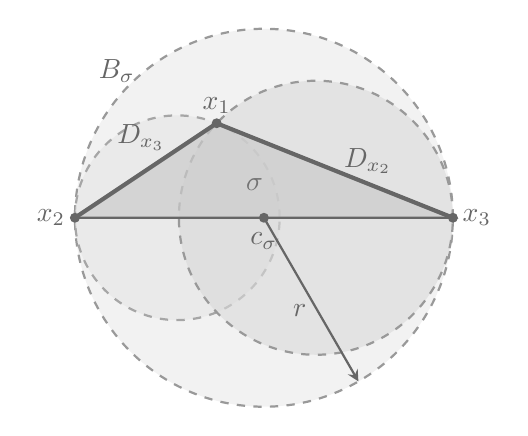
\begin{tikzpicture}[scale=1.2]
        % Coordonnées
        \coordinate (M) at (0,0);
        \coordinate (X2) at (-2,0);
        \coordinate (X3) at (2,0);
        
        % x_1 (anciennement a) est décalé pour casser la symétrie du triangle isocèle
        \coordinate (X1) at (-0.5,1);

        % Centres et rayons des disques de Delaunay D_{x_3} et D_{x_2}
        % Calculés géométriquement pour passer par X1(-0.5, 1) et être tangents en X2(-2,0) et X3(2,0)
        \coordinate (Cx3) at (-0.9167, 0);
        \def\Rtrois{1.0833}
        
        \coordinate (Cx2) at (0.55, 0);
        \def\Rdeux{1.45}

        % Boule minimale B_sigma (Diamètre [x_2, x_3])
        \fill[gray!10] (M) circle (2);
        \draw[dashed, gray!80, thick] (M) circle (2);
        \node[gray!80!black] at (135:2.2) {$B_\sigma$};

        % Disque vide D_{x_3} pour l'arête [x_1,x_2] (à gauche)
        \fill[gray!20, fill opacity=0.6] (Cx3) circle (\Rtrois);
        \draw[dashed, gray!70, thick] (Cx3) circle (\Rtrois);
        \node[gray!80!black] at (-1.3, 0.85) {$D_{x_3}$};

        % Disque vide D_{x_2} pour l'arête [x_1,x_3] (à droite)
        \fill[gray!30, fill opacity=0.6] (Cx2) circle (\Rdeux);
        \draw[dashed, gray!80, thick] (Cx2) circle (\Rdeux);
        \node[gray!80!black] at (1.1, 0.6) {$D_{x_2}$};

        % Triangle obtus (Fond)
        \fill[gray!40, fill opacity=0.7] (X2) -- (X3) -- (X1) -- cycle;
        \draw[thick, gray!80!black] (X2) -- (X3) -- (X1) -- cycle;
        \node[gray!90!black] at (-0.1, 0.35) {$\sigma$};
        
        % Les arêtes de Delaunay mises en évidence
        \draw[line width=1.5pt, gray!80!black] (X2) -- (X1);
        \draw[line width=1.5pt, gray!80!black] (X3) -- (X1);

        % Rayon et centre de la boule minimale
        \draw[->, >=stealth, gray!80!black, thick] (M) -- (-60:2) node[midway, below left=-2pt] {$r$};
        \fill[gray!80!black] (M) circle (1.5pt) node[below=2pt] {$c_\sigma$};

        % Sommets
        \fill[gray!80!black] (X2) circle (1.5pt) node[left] {$x_2$};
        \fill[gray!80!black] (X3) circle (1.5pt) node[right] {$x_3$};
        \fill[gray!80!black] (X1) circle (1.5pt) node[above] {$x_1$};

    \end{tikzpicture}
    \caption{Illustration de la preuve de \Fact~\ref{fait:opt_K2_gabriel}. Si un triangle obtus $\sigma=\{x_1,x_2,x_3\}$ est de \nom{Gabriel}, sa boule minimale $B_\sigma$ de diamètre $[x_2,x_3]$ est vide de tout ``intrus''. L'on peut alors y inscrire deux disques $D_{x_3}$ et $D_{x_2}$ inclus dans $B_\sigma$ (et donc également vides de tout point de $\mathcal X$). Ces disques vides attestent que $[x_1,x_2]$ et $[x_1,x_3]$ sont bien de \nom{Delaunay}.}
    \label{fig:chapV_gabriel_obtus}
\end{figure}



\subsection{Digression au cas $K \ge 2$}


Ces idées (\Fact~\ref{fait:opt_K2_gabriel} et la preuve) se généralisent très bien pour $K \ge 2$.
%Pour les \(K\)-polyèdres, les sommets du graphe dual \(\Gamma_K\) sont des \((K-1)\)-simplexes, c'est-à-dire des sous-ensembles de \(X\) de cardinal \(K\), et les fusions élémentaires sont portées par des \(K\)-simplexes, c'est-à-dire des sous-ensembles de cardinal \(K+1\).

La mosaïque de \textsc{Delaunay} \(\mathrm{Del}_{K-1}(\mathcal X)\) d'ordre \(K-1\) a pour sommets les sous-ensembles
\(Q \subset \mathcal X\) de cardinal \(K-1\) associés à une cellule de \textsc{Voronoï} d'ordre \(K-1\) non vide. Les arêtes élémentaires de cette mosaïque (reliant deux sommets \(Q,Q'\) tels que
\(
        |Q \cup Q'| = K,
\))
portent donc un \((K-1)\)-simplexe
\(
        \tau = Q \cup Q' .
\)

Autrement dit, les arêtes élémentaires de \(\mathrm{Del}_{K-1}(X)\)
fournissent des candidats pour les sommets de \(\Gamma_K(\mathcal X)\).

Regardons à présent les arêtes de \(\Gamma_K(\mathcal X)\) : soit \(\sigma \subseteq \X\) un \(K\)-simplexe de \textsc{Gabriel}, \(|\sigma|=K+1\). Notons comme à l'accoutumée
\(
        B_\sigma = B(c_\sigma,\rho(\sigma))
\)
sa plus petite boule englobante, et
\(
        S = \sigma \cap \partial B_\sigma
\)
son ensemble de support. Comme \(B_\sigma\) est minimale, on a
\(|S|\geq 2\). Pour tout \(s\in S\), on pose
\(
        \tau_s = \sigma \setminus \{s\}.
\)
Alors chaque facette active \(\tau_s\) est portée par la mosaïque
\(\mathrm{Del}_{K-1}(\mathcal X)\) : par les arguments maintenant habituels (\Res~\ref{res:chapIV_miniball_support}), il existe deux sommets adjacents
\(Q,Q'\) de \(\mathrm{Del}_{K-1}(\mathcal X)\) tels que
\(
        Q\cup Q' = \tau_s .
\) 


%En effet, si \(|S|\geq 3\), le centre \(c_\sigma\) de la boule minimale témoigne directement de cette propriété : les points de \(\sigma\cap \mathring B_\sigma\) sont strictement plus proches de \(c_\sigma\), tandis que les points de \(S\) sont à distance égale. Après avoir retiré \(s\), il reste au moins deux points de support dans \(\tau_s\), ce qui donne deux choix distincts de \(K-1\) plus proches voisins dont l'union est \(\tau_s\).

% Si \(|S|=2\), écrivons \(S=\{s,t\}\). On considère alors les boules fermées contenues dans \(B_\sigma\), tangentes à \(B_\sigma\) au point \(t\), obtenues en déplaçant légèrement le centre \(c_\sigma\) vers \(t\) et en diminuant le rayon d'autant. Pour un déplacement nul, tous les points de \(\tau_s\) sont contenus dans la boule. Pour un déplacement maximal admissible, la boule contient encore \(\tau_s\), elle est tangente en \(t\), et au moins un autre point de \(\tau_s\) appartient à sa frontière. Elle ne contient aucun point de \(X\setminus \sigma\), puisqu'elle est incluse dans \(B_\sigma\), et elle ne contient pas \(s\). Son centre appartient donc à l'intersection de deux cellules de Voronoï d'ordre \(K-1\), associées à deux \((K-1)\)-uplets dont l'union est \(\tau_s\). Ainsi \(\tau_s\) est bien portée par une arête élémentaire de \(\mathrm{Del}_{K-1}(X)\).

Comme \(|S|\geq 2\), en choisissant deux points distincts \(s,t\in S\),
on obtient deux facettes actives
\[
        \tau_s = \sigma\setminus\{s\},
        \qquad
        \tau_t = \sigma\setminus\{t\},
\]
et leur union redonne le simplexe entier :
\[
        \tau_s \cup \tau_t = \sigma .
\]
Par conséquent, on obtient le résultat suivant généralisant \Fact~\ref{fait:opt_K2_gabriel} à $K\ge 2$.
\begin{Theoreme}{Le $K$-graphe de \textsc{Gabriel} se lit dans la mosaïque de \textsc{Delaunay} \(\mathrm{Del}_{K-1}\) d'ordre $K-1$}{KGabriel_depuis_KM1Delaunay}
Tout \(K\)-simplexe de \nom{Gabriel} peut être identifié à partir de deux \((K-1)\)-simplexes portés par des arêtes élémentaires de \(\mathrm{Del}_{K-1}(X)\).
\end{Theoreme}


Ce \Th~\ref{th:KGabriel_depuis_KM1Delaunay} permet le résultat algorithmique suivant : pour retrouver la hiérarchie complète des niveaux $K$-NN, il suffit\footnote{Il y a tout de même un coût supplémentaire non négligeable en grande dimension : trouver le rayon de filtration $r_\sigma$ des simplexes $\sigma$ candidats, par exemple au moyen de l'algorithme de \textsc{Welzl} \cite{Welzl1991} (et éventuellement tester qu'ils sont bien de \textsc{Gabriel}).} de construire la mosaïque \(\mathrm{Del}_{K-1}(X)\) d'ordre $K-1$.
% \((K-1)\)-simplexes candidats, former les unions de deux tels candidats
% dont l'union a cardinal \(K+1\), puis ne conserver que les unions
% \(\sigma\) qui satisfont le test Gabriel, c'est-à-dire
% \[
%         \mathring B_\sigma \cap (X\setminus \sigma)=\varnothing .
% \]
% Une fois un \(K\)-simplexe Gabriel \(\sigma\) identifié, on insère dans
% le graphe dual toutes ses facettes, y compris celles qui ne sont pas
% nécessairement visibles comme arêtes de \(\mathrm{Del}_{K-1}(X)\).



\subsection{L'algorithme pour $K=2$}

\Fact~\ref{fait:opt_K2_gabriel} permet d'obtenir \Fact~\ref{fait:chapV_k2_gabriel_plan} ainsi que l'\Alg~\ref{alg:chapV_hgp_k2} utilisé dans la suite de ce chapitre sur les données expérimentales. 

\begin{Fait}{Extraction planaire du \(2\)-graphe de \nom{Gabriel} \cite{BibiAppliedNetworkScience}}{chapV_k2_gabriel_plan}
Soit $\X\subset\mathbb R^2$ un nuage fini en position générale. Tous les triangles de \nom{Gabriel} de $\X$ peuvent être extraits à partir de la triangulation de \nom{Delaunay} ordinaire de $\X$. En particulier, le graphe dual des arêtes reliées par les triangles de \nom{Gabriel} peut être construit en temps $\mathcal O(n\log n)$ dans le plan.
\end{Fait}



\begin{algorithm}[htbp]
  \caption{\textsc{HGP-Clusterer} pour $K=2$ avec sortie en partition stricte}\label{alg:chapV_hgp_k2}
  \textbf{Entrée :} Nuage de points $\X\subset\mathbb R^p$, seuil \texttt{min\_cluster\_size}, choix de poids $\psi$\\
  \textbf{Sortie :} Clustering sur $\X$
  \begin{algorithmic}[1]
    \State Construire la triangulation de \nom{Delaunay} $\mathrm{Del}(\mathcal X)$.
    \State Extraire les triangles de \nom{Gabriel} : triangles aigus de $\mathrm{Del}(\X)$ satisfaisant le test de vacuité, puis triangles obtus énumérés à partir des couples d'arêtes de \nom{Delaunay} incidentes (voir \Fact~\ref{fait:opt_K2_gabriel}).
    \State Construire le graphe dual $G_2$ dont les sommets sont les arêtes $\tau=\{x_i,x_j\}$ apparaissant comme facettes d'au moins un triangle de \nom{Gabriel}.
    \State Pour chaque triangle $\sigma=\{x_i,x_j,x_k\}$, relier (deux de) ses trois arêtes-facettes dans $G_2$ avec une fusion de poids $\rho(\sigma)$.
    \State Calculer les scores de faces $S_\tau=\sum_{\sigma\supset\tau}\psi(\rho(\sigma))$ et les masses $m_\tau=S_\tau\sum_{x\in\tau}T_x^{-1}$.
    \State Extraire un arbre couvrant minimal $T_2$ de $G_2$ par \textsc{Kruskal}.
    \State Condenser $T_2$ avec le seuil \texttt{min\_cluster\_size} \cite{HDBSCAN2017} et sélectionner les clusters par excès de masse.
    \State Propager les étiquettes des clusters aux points par le vote pondéré (voir la section précédente).
    \State Optionnellement, réaffecter les points non classés par $1$-plus proche voisin parmi les points déjà étiquetés.
  \end{algorithmic}
\end{algorithm}


\Remarque{En dimension plus grande, la mise en \oe uvre exacte devient rapidement limitée par la construction de la mosaïque de \nom{Delaunay} d'ordre $K$. Des approximations de type \nom{Rips}, une réduction préalable de dimension, un sous-échantillonnage suivi d'une propagation par $k$-plus proches voisins, ou encore une recherche restreinte à des listes de voisins sont des options praticables. Elles doivent toutefois être distinguées de la construction géométrique exacte : dès qu'une approximation remplace la mosaïque exacte, les garanties d'équivalence avec les $K$-polyèdres exacts ne valent plus sans hypothèses supplémentaires.}

\subsection{Résultats sur les huiles d'olive italiennes}
\label{subsec:chapV_huiles_olive}

Le jeu de données des huiles d'olive italiennes \cite{HuileOlive} contient $572$ échantillons, chacun décrit par huit concentrations en acides gras. 
Ainsi le nuage $\mathcal X \subset \mathbb R^8$ est représenté par une matrice de taille $572 \times 8$.
Comme dans \cite{DegreeRipsRolleScoccola}, nous avons centré puis normalisé (en norme $\ell^2$) les colonnes de la matrice.
Les données ont été mises à disposition publiquement par \cite{DonneesHuileOlive}. Les échantillons proviennent de neuf provinces italiennes, regroupées en trois macro-régions : Italie du Sud, Sardaigne, puis Centre-Nord. 


HDBSCAN retrouve correctement les trois macro-régions, mais ne sépare pas les neuf provinces fines. La méthode \nom{Persistable} de \cite{DegreeRipsRolleScoccola} est l'état-de-l'art pour l'identification des plus petites provinces : elle retrouve huit des neuf provinces (la Sicile n'est pas identifiée), mais ne classe directement que $279$ points, soit environ $49\%$ des données. Notre méthode \cite{BibiAppliedNetworkScience} avec $K=2$ retrouve également huit groupes interprétables (et c'est encore la Sicile qui échappe à l'identification, absorbée par les groupes de Calabre et de Pouilles du Nord), mais elle classe directement $412$ points, soit environ $72\%$ des données, avec $396/412\approx96.1\%$ d'étiquettes correctes.

Dans les deux tableaux suivants (\Tab~\ref{tab:chapV_italie_partiel} \& \Tab~\ref{tab:chapV_italie_exhaustif}), chaque case contient le résultat de \nom{Persistable}, puis celui de HGP-Clusterer. La colonne $4$ correspond à la Sicile, non identifiée.

\begin{table}[htbp]
\centering
\caption{Résultats partiels de \nom{Persistable} et de HGP-Clusterer sur le jeu de données des huiles d'olive italiennes. La notation $a/ b$ indique \nom{Persistable}/HGP-Clusterer.}
\label{tab:chapV_italie_partiel}
% \begingroup
\small
\setlength{\tabcolsep}{2pt}
% \resizebox{\textwidth}{!}{%
\begin{tabular}{@{}l*{9}{c}c@{}}
\toprule
\textbf{\nom{Pers.}/HGP} & \textbf{1} & \textbf{2} & \textbf{3} & \textbf{4} &
\textbf{5} & \textbf{6} & \textbf{7} & \textbf{8} & \textbf{9} & \textbf{{\footnotesize Non classés}} \\
\midrule
{\color[HTML]{CB0000}\textbf{N.\,Apulia}}
  & 12/\textbf{24} & {\color[HTML]{C0C0C0}0/0} & {\color[HTML]{C0C0C0}0/0} & -- %
  & {\color[HTML]{C0C0C0}0/0} & {\color[HTML]{C0C0C0}0/0} & {\color[HTML]{C0C0C0}0/0}
  & {\color[HTML]{C0C0C0}0/0} & {\color[HTML]{C0C0C0}0/0} & 13/\textbf{1} \\
\cmidrule(lr){2-11}
{\color[HTML]{FE0000}\textbf{Calabria}}
  & {\color[HTML]{C0C0C0}0/0} & 7/\textbf{25} & \textbf{1}/2 & -- %
  & {\color[HTML]{C0C0C0}0/0} & {\color[HTML]{C0C0C0}0/0} & {\color[HTML]{C0C0C0}0/0}
  & {\color[HTML]{C0C0C0}0/0} & {\color[HTML]{C0C0C0}0/0} & 48/\textbf{29} \\
\cmidrule(lr){2-11}
{\color[HTML]{680100}\textbf{S.\,Apulia}}
  & {\color[HTML]{C0C0C0}0/0} & {\color[HTML]{C0C0C0}0/0} & 100/\textbf{145} & -- %
  & {\color[HTML]{C0C0C0}0/0} & {\color[HTML]{C0C0C0}0/0} & {\color[HTML]{C0C0C0}0/0}
  & {\color[HTML]{C0C0C0}0/0} & {\color[HTML]{C0C0C0}0/0} & 106/\textbf{61} \\
\cmidrule(lr){2-11}
{\color[HTML]{FD6864}\textbf{Sicilia}}
  & \textbf{3}/6 & \textbf{0}/2 & \textbf{0}/1 & -- %
  & {\color[HTML]{C0C0C0}0/0} & {\color[HTML]{C0C0C0}0/0} & {\color[HTML]{C0C0C0}0/0}
  & {\color[HTML]{C0C0C0}0/0} & {\color[HTML]{C0C0C0}0/0} & \textbf{33}/27 \\
\midrule
{\color[HTML]{7B7B7B}\textbf{Inl.\,Sard.}}
  & {\color[HTML]{C0C0C0}0/0} & {\color[HTML]{C0C0C0}0/0} & {\color[HTML]{C0C0C0}0/0}
  & -- & 51/\textbf{62} & {\color[HTML]{C0C0C0}0/0}
  & {\color[HTML]{C0C0C0}0/0} & {\color[HTML]{C0C0C0}0/0} & {\color[HTML]{C0C0C0}0/0}
  & 14/\textbf{3} \\
\cmidrule(lr){2-11}
{\color[HTML]{2F2F2F}\textbf{Coast S.}}
  & {\color[HTML]{C0C0C0}0/0} & {\color[HTML]{C0C0C0}0/0} & {\color[HTML]{C0C0C0}0/0}
  & -- & \textbf{0}/2 & 19/\textbf{29} & {\color[HTML]{C0C0C0}0/0}
  & {\color[HTML]{C0C0C0}0/0} & {\color[HTML]{C0C0C0}0/0} & 14/\textbf{2} \\
\midrule
{\color[HTML]{32CB00}\textbf{E.\,Ligur.}}
  & {\color[HTML]{C0C0C0}0/0} & {\color[HTML]{C0C0C0}0/0} & {\color[HTML]{C0C0C0}0/0}
  & -- & {\color[HTML]{C0C0C0}0/0} & {\color[HTML]{C0C0C0}0/0} & 14/\textbf{32}
  & \textbf{1}/2 & \textbf{0}/1 & 35/\textbf{15} \\
\cmidrule(lr){2-11}
{\color[HTML]{34FF34}\textbf{W.\,Ligur.}}
  & {\color[HTML]{C0C0C0}0/0} & {\color[HTML]{C0C0C0}0/0} & {\color[HTML]{C0C0C0}0/0}
  & -- & {\color[HTML]{C0C0C0}0/0} & {\color[HTML]{C0C0C0}0/0} & {\color[HTML]{C0C0C0}0/0}
  & 29/\textbf{33} & {\color[HTML]{C0C0C0}0/0} & 21/\textbf{17} \\
\cmidrule(lr){2-11}
{\color[HTML]{036400}\textbf{Umbria}}
  & {\color[HTML]{C0C0C0}0/0} & {\color[HTML]{C0C0C0}0/0} & {\color[HTML]{C0C0C0}0/0}
  & -- & {\color[HTML]{C0C0C0}0/0} & {\color[HTML]{C0C0C0}0/0} & {\color[HTML]{C0C0C0}0/0}
  & {\color[HTML]{C0C0C0}0/0} & 42/\textbf{46} & 9/\textbf{5} \\
\bottomrule
\end{tabular}%
% }
% \endgroup
\end{table}

L'extension exhaustive par $1$-plus proche voisin des points non classés donne $521/572\approx91,1\%$ d'étiquettes correctes et un indice de \nom{Rand} ajusté \cite{AdjustedRandIndex} (\emph{Adjusted Rand Index}, ARI, en anglais) égal à $0,890$. La version exhaustive de \nom{Persistable} atteint $499/572\approx87,2\%$ et un ARI égal à $0,848$.

\begin{table}[htbp]
\centering
\caption{Résultats exhaustifs de \nom{Persistable} et de HGP-Clusterer sur le jeu de données des huiles d'olive italiennes, après propagation aux points non classés. La notation $a/ b$ indique \nom{Persistable}/HGP-Clusterer.}
\label{tab:chapV_italie_exhaustif}
% \begingroup
\small
\setlength{\tabcolsep}{2pt}
% \resizebox{\textwidth}{!}{%
\begin{tabular}{@{}l*{9}{c}c@{}}
\toprule
\textbf{\nom{Pers.}/HGP} & \textbf{1} & \textbf{2} & \textbf{3} & \textbf{4} &
\textbf{5} & \textbf{6} & \textbf{7} & \textbf{8} & \textbf{9} & \textbf{{\footnotesize Non classés}}\\
\midrule
{\color[HTML]{CB0000}\textbf{N.\,Apulia}}
  & 21/\textbf{24} & 2/\textbf{1} & {\color[HTML]{C0C0C0}0/0} & -- %
  & {\color[HTML]{C0C0C0}0/0} & {\color[HTML]{C0C0C0}0/0} & {\color[HTML]{C0C0C0}0/0}
  & {\color[HTML]{C0C0C0}0/0} & {\color[HTML]{C0C0C0}0/0} & 2/\textbf{0}\\
\cmidrule(lr){2-11}
{\color[HTML]{FE0000}\textbf{Calabria}}
  & \textbf{0}/1 & 50/\textbf{52} & 3/\textbf{2} & -- %
  & {\color[HTML]{C0C0C0}0/0} & {\color[HTML]{C0C0C0}0/0} & \textbf{1}/\textbf{1}
  & {\color[HTML]{C0C0C0}0/0} & {\color[HTML]{C0C0C0}0/0} & 2/\textbf{0}\\
\cmidrule(lr){2-11}
{\color[HTML]{680100}\textbf{S.\,Apulia}}
  & \textbf{0}/2 & 1/\textbf{0} & 196/\textbf{204} & -- %
  & {\color[HTML]{C0C0C0}0/0} & {\color[HTML]{C0C0C0}0/0} & {\color[HTML]{C0C0C0}0/0}
  & {\color[HTML]{C0C0C0}0/0} & {\color[HTML]{C0C0C0}0/0} & 9/\textbf{0}\\
\cmidrule(lr){2-11}
{\color[HTML]{FD6864}\textbf{Sicilia}}
  & \textbf{6}/10 & 20/\textbf{16} & \textbf{7}/10 & -- %
  & {\color[HTML]{C0C0C0}0/0} & {\color[HTML]{C0C0C0}0/0} & {\color[HTML]{C0C0C0}0/0}
  & {\color[HTML]{C0C0C0}0/0} & {\color[HTML]{C0C0C0}0/0} & \textbf{3}/0\\
\midrule
{\color[HTML]{7B7B7B}\textbf{Inl.\,Sard.}}
  & {\color[HTML]{C0C0C0}0/0} & {\color[HTML]{C0C0C0}0/0} & {\color[HTML]{C0C0C0}0/0}
  & -- & \textbf{65}/\textbf{65} & {\color[HTML]{C0C0C0}0/0}
  & {\color[HTML]{C0C0C0}0/0} & {\color[HTML]{C0C0C0}0/0} & {\color[HTML]{C0C0C0}0/0}
  & {\color[HTML]{C0C0C0}0/0}\\
\cmidrule(lr){2-11}
{\color[HTML]{2F2F2F}\textbf{Coast S.}}
  & {\color[HTML]{C0C0C0}0/0} & {\color[HTML]{C0C0C0}0/0} & {\color[HTML]{C0C0C0}0/0}
  & -- & \textbf{2}/\textbf{2} & \textbf{31}/\textbf{31}
  & {\color[HTML]{C0C0C0}0/0} & {\color[HTML]{C0C0C0}0/0} & {\color[HTML]{C0C0C0}0/0}
  & {\color[HTML]{C0C0C0}0/0}\\
\midrule
{\color[HTML]{32CB00}\textbf{E.\,Ligur.}}
  & {\color[HTML]{C0C0C0}0/0} & {\color[HTML]{C0C0C0}0/0} & {\color[HTML]{C0C0C0}0/0}
  & -- & {\color[HTML]{C0C0C0}0/0} & {\color[HTML]{C0C0C0}0/0} & 41/\textbf{44}
  & \textbf{2}/5 & \textbf{0}/1 & 7/\textbf{0}\\
\cmidrule(lr){2-11}
{\color[HTML]{34FF34}\textbf{W.\,Ligur.}}
  & {\color[HTML]{C0C0C0}0/0} & {\color[HTML]{C0C0C0}0/0} & {\color[HTML]{C0C0C0}0/0}
  & -- & {\color[HTML]{C0C0C0}0/0} & {\color[HTML]{C0C0C0}0/0} & {\color[HTML]{C0C0C0}0/0}
  & 47/\textbf{50} & {\color[HTML]{C0C0C0}0/0} & 3/\textbf{0}\\
\cmidrule(lr){2-11}
{\color[HTML]{036400}\textbf{Umbria}}
  & {\color[HTML]{C0C0C0}0/0} & {\color[HTML]{C0C0C0}0/0} & {\color[HTML]{C0C0C0}0/0}
  & -- & {\color[HTML]{C0C0C0}0/0} & {\color[HTML]{C0C0C0}0/0} & 2/\textbf{0}
  & {\color[HTML]{C0C0C0}0/0} & 48/\textbf{51} & 1/\textbf{0}\\
\bottomrule
\end{tabular}%
% }
% \endgroup
\end{table}

\subsection{Résultats sur SIPU}
\label{subsec:chapV_sipu}

Le \emph{benchmark} public SIPU \cite{Sipu}, utilisé ici \emph{via} \nom{ClustBench} \cite{Clustbench}, regroupe des jeux de données synthétiques de formes et de tailles très variées. Les jeux admettant une vérité terrain multiple -- et donc sujette à ambiguïté --, comme \texttt{compound}, \texttt{flame}, \texttt{pathbased} et \texttt{r15}, n'ont pas été retenus ; \texttt{worms\_64} est également écarté à cause de sa dimension $64$ (du fait du fléau de la dimension, la triangulation de \textsc{Delaunay} n'est pas calculable).

La comparaison avec HDBSCAN \cite{HDBSCAN2017} est rigoureusement faite : on garde le même seuil minimal de percolation, \texttt{min\_cluster\_size}$=\sqrt n$, le même estimateur de densité $\widehat\rho=1/r$%
, et le même critère d'excès de masse ($\psi(t) = \tfrac1t$). Toutes choses égales par ailleurs, la seule différence est donc le type de connexité : connexité standard de graphe géométrique pour HDBSCAN, connexité par triangles de \v Cech pour HGP-Clusterer avec $K=2$ \cite{BibiAppliedNetworkScience}.

\begin{table}[htbp]
\centering
\caption{Résultats de HDBSCAN et de HGP-Clusterer sur les jeux de données SIPU. $n$ désigne la taille du jeu de données, $k$ le nombre de clusters, ARI l'indice de \nom{Rand} ajusté, et ``classés'' la proportion de points affectés à un cluster.}
\small
\label{tab:chapV_sipu}
\begin{tabular}{@{}lrrrrrrrr@{}}
\toprule
\multicolumn{3}{c}{\textbf{Vérité terrain}} &
\multicolumn{3}{c}{\textbf{HDBSCAN}} &
\multicolumn{3}{c}{\textbf{HGP-Clusterer}} \\
\cmidrule(lr){1-3}\cmidrule(lr){4-6}\cmidrule(lr){7-9}
\textbf{Jeu} & $n$ & $k$ & $k$ & ARI & Classés & $k$ & ARI & Classés \\
\midrule
a1 & 3\,000 & 20 & \textbf{17} & 0.745 & 94.9\% & \textbf{17} & \textbf{0.778} & \textbf{97.7\%}\\
a2 & 5\,250 & 35 & \textbf{33} & 0.762 & 92.1\% & 32 & \textbf{0.834} & \textbf{96.2\%} \\
a3 & 7\,500 & 50 & 43 & 0.696 & 95.0\% & \textbf{45} & \textbf{0.831} & \textbf{97.1\%} \\
aggregation & 788 & 7 & \textbf{5} & \textbf{0.809} & \textbf{100.0\%} & \textbf{5} & \textbf{0.809} & \textbf{100.0\%} \\
birch1 & 100\,000 & 100 & 98 & 0.215 & 79.7\% & \textbf{100} & \textbf{0.298} & \textbf{83.1\%} \\
birch2 & 100\,000 & 100 & \textbf{100} & \textbf{0.996} & \textbf{99.7\%} & 84 & 0.441 & 83.9\% \\
d31 & 3\,100 & 31 & 27 & 0.659 & 90.0\% & \textbf{30} & \textbf{0.835} & \textbf{94.5\%} \\
jain & 373 & 2 & \textbf{3} & \textbf{0.935} & 98.4\% & \textbf{3} & \textbf{0.935} & \textbf{98.7\%} \\
s1 & 5\,000 & 15 & \textbf{15} & 0.961 & 97.6\% & \textbf{15} & \textbf{0.976} & \textbf{99.0\%} \\
s2 & 5\,000 & 15 & \textbf{15} & 0.783 & 88.9\% & \textbf{15} & \textbf{0.842} & \textbf{91.9\%} \\
s3 & 5\,000 & 15 & \textbf{15} & 0.251 & 65.9\% & \textbf{15} & \textbf{0.418} & \textbf{77.2\%} \\
s4 & 5\,000 & 15 & \textbf{15} & 0.258 & 67.4\% & \textbf{15} & \textbf{0.284} & \textbf{69.6\%} \\
spiral & 312 & 3 & \textbf{3} & \textbf{1.000} & \textbf{100.0\%} & \textbf{3} & \textbf{1.000} & \textbf{100.0\%} \\
unbalance & 6\,500 & 8 & \textbf{8} & \textbf{1.000} & 99.9\% & \textbf{8} & \textbf{1.000} & \textbf{100.0\%} \\
worms\_2 & 105\,600 & 35 & 15 & 0.055 & \textbf{74.2\%} & \textbf{33} & \textbf{0.076} & 66.4\% \\
\bottomrule
\end{tabular}%
\end{table}

Les résultats sont en \Tab~\ref{tab:chapV_sipu}. HGP-Clusterer améliore nettement l'ARI sur la plupart des jeux difficiles, en particulier \texttt{a2}, \texttt{a3}, \texttt{d31}, \texttt{s2} et \texttt{s3}. Il classe aussi une proportion plus grande de points dans la plupart des cas, parce que la connexité triangulaire évite de construire des filaments instables (créant des ``trous'' dont les points à l'intérieur sont ``perdus''). Une exception cependant : \texttt{birch2}, où HDBSCAN est presque parfait et où HGP-Clusterer fusionne intempestivement certains clusters. La raison en est que les clusters sont essentiellement filiformes et sont donc mieux identifiés avec de simples graphes. À noter que poser le bon estimateur $\widehat\rho=1/r^2$ résout le problème et HGP-Clusterer devient alors quasi-parfait pour identifier le bon nombre de clusters. %\footnote{Alors qu'en dimension 2 et avec $K=2$, il est plus exact de prendre $\widehat\rho=1/r^2$ ; les résultats de HGP-Clusterer étant d'ailleurs meilleurs ce faisant, notamment pour retrouver le nombre exact de clusters.}.



\section{Lorsque la mosaïque de \nom{Delaunay} n'est plus disponible : le complexe de \nom{Vietoris}--\nom{Rips}}
\label{sec:chapV_vietoris_rips}

La construction exacte des chapitres précédents repose sur le complexe de \v Cech, puis sur son amincissement par la mosaïque de \nom{Delaunay} d'ordre $K$ et le $K$-graphe de \nom{Gabriel}. C'est la bonne voie -- tant théorique que pratique -- lorsque les données sont effectivement un nuage euclidien de dimension modérée (et que le modèle de \textsc{Hartigan} est pertinent). Mais il existe des situations où cette voie n'est plus possible.

D'abord, lorsque les données ne sont pas dans l'espace euclidien $\mathbb R^p$. L'on peut, \emph{exempli gratia}, ne disposer que d'une matrice de distances, éventuellement creuse (ou \emph{sparse} en anglais). 
Dans ces cas, toutes les notions de boules minimales, de cellule de \nom{Voronoï} ou de mosaïque de \nom{Delaunay} tombent.

Une seconde raison est algorithmique : même lorsque les données sont euclidiennes, la grande dimension rend la mosaïque de \nom{Delaunay} rapidement incalculable en pratique. La triangulation de \nom{Delaunay} ordinaire peut déjà avoir une complexité au pire cas $\mathcal O(n^{\lceil p/2\rceil})$ dans $\mathbb R^p$ \cite{BoissonnatChazalYvinec}. %À l'ordre $K$, l'explosion combinatoire arrive encore plus vite. 
Il faut donc faire appel à des constructions de remplacement qui permettent de faire tourner l'algorithme dans des cadres moins favorables. Le complexe de \nom{Vietoris}--\nom{Rips} est une possibilité assez naturelle.

\begin{Definition}{Complexe de \nom{Vietoris}--\nom{Rips} \cite{Munkres, BoissonnatChazalYvinec}}{chapV_vietoris_rips_complexe}
Soit $(\X,d)$ un espace métrique fini et soit $r\ge0$. Le complexe de \nom{Vietoris}--\nom{Rips} de rayon $r$ est le complexe simplicial
\[
\boxed{
    \mathrm{VR}(\X,r)
    \eqdef
    \left\{
        \sigma\subseteq \X
        \ \middle|\
        \forall x,x'\in\sigma,\ d(x,x')\le 2r
    \right\}.
    }
\]
Autrement dit, $\sigma$ est un simplexe de $\mathrm{VR}(\X,r)$ si et seulement si tous ses sommets sont deux à deux reliés dans le graphe seuil
\[
    G_r=(\X,E_r),
    \qquad
    E_r\eqdef
    \bigl\{\{x,x'\}\subseteq\X\mid d(x,x')\le 2r\bigr\}.
\]
\end{Definition}
\Remarque{Les complexes de \v Cech et \textsc{Vietoris--Rips} ont même $1$-squelette (graphe sous-jacent) : le graphe géométrique seuil. De plus, le complexe de \nom{Vietoris}--\nom{Rips} est le plus grand complexe constructible sur ce graphe seuil (dès qu'une clique est présente, le simplexe associé apparaît) ; on dit qu'il est le complexe de drapeau (ou \emph{flag complex} en anglais) du graphe géométrique $G_r$.}

% Elle admet aussi une version purement graphée : si l'entrée est un graphe pondéré $G=(\X,E,w)$, on pose
% \[
%     \mathrm{VR}(G,r)
%     \eqdef
%     \left\{
%         \sigma\subseteq \X
%         \ \middle|\
%         \forall x\neq x'\in\sigma,\ \{x,x'\}\in E
%         \ \mathrm{et}\ 
%         w(x,x')\le 2r
%     \right\}.
% \]
L'on pourrait tout à fait définir de façon plus générale le complexe de \textsc{Vietoris--Rips} sur un graphe pondéré en considérant que les arêtes absentes ont un poids $+\infty$ pour pouvoir ainsi travailler avec des matrices de distance creuses.


\begin{Resultat}{Encadrement \v Cech--\nom{Rips} dans $\mathbb R^p$ \cite{BoissonnatChazalYvinec}}{chapV_cech_rips_intercalage}
Soit $\X\subset\mathbb R^p$ un nuage localement fini. Pour tout $r\ge0$,
\[
\boxed{
    \check C(\X,r)
    \subseteq
    \mathrm{VR}(\X,r)
    \subseteq
    \check C\!\left(\X,\alpha_p r\right),}
    \qquad
    \alpha_p\eqdef \sqrt{\frac{2p}{p+1}}\le\sqrt2.
\]
En particulier, tout $K$-polyèdre de $\check C(\X,r)$ est contenu dans un $K$-polyèdre de $\mathrm{VR}(\X,r)$, et tout $K$-polyèdre de $\mathrm{VR}(\X,r)$ est contenu dans un $K$-polyèdre de $\check C(\X,\alpha_p r)$.
\end{Resultat}
\begin{preuve}
La première inclusion est immédiate : les complexes ont même $1$-squelette, et le complexe de \textsc{Vietoris--Rips} est le plus grand possible (\emph{flag complex}). La seconde inclusion est une conséquence du théorème de \nom{Jung} \cite{jung1901kleinste} : un ensemble de diamètre au plus $2r$ dans $\mathbb R^p$ est contenu dans une boule de rayon au plus $\alpha_p r$.
\end{preuve}

Le \Res~\ref{res:chapV_cech_rips_intercalage} permet de voir en le complexe de \textsc{Vietoris--Rips} une approximation contrôlée du complexe de \v Cech dans le cas euclidien. À noter que cette approximation devient cependant de plus en plus mauvaise au fur et à mesure que la dimension $p$ croît.

Le complexe de \textsc{Vietoris--Rips} fournit aussi une extension naturelle pour le cas métrique général.

\begin{Fait}{Les $K$-polyèdres de \nom{Rips} comme percolation de cliques}{chapV_rips_clique_percolation}
Fixons $r\ge0$ et notons $G_r$ le graphe seuil associé à $\mathrm{VR}(\X,r)$. Les $K$-simplexes de $\mathrm{VR}(\X,r)$ sont exactement les cliques de taille $K+1$ de $G_r$.

Les $K$-polyèdres non triviaux de $\mathrm{VR}(\X,r)$ correspondent donc aux usuelles composantes de \emph{clique percolation} \cite{KCliquePercolation}.
\end{Fait}


L'intérêt pratique majeur de \nom{Vietoris--Rips} est qu'il ouvre la porte à des implémentations massivement parallèles, en particulier sur \textsc{GPU}. La géométrie euclidienne exacte disparaît au profit de quatre opérations de graphes, dont les trois premières (qui représentent le coût véritable de l'algorithme) sont massivement parallélisables.

\begin{enumerate}
    \item \textbf{Construction du graphe de voisinage.} Si les données sont euclidiennes mais de grande dimension, on peut construire un graphe (approché) de voisinages. Cette étape se parallélise naturellement. Si l'entrée est déjà une matrice creuse (\emph{sparse} en anglais), cette étape est simplement sautée.

    \item \textbf{Énumération des cliques.} Pour $K=2$, il suffit d'énumérer les triangles du graphe. C'est le cas le plus favorable : les triangles se calculent par intersections de listes d'adjacence triées. Pour $K$ fixé plus grand, on peut énumérer les $(K+1)$-cliques par intersections récursives de voisinages. La complexité dépend alors du nombre réel de cliques du graphe parcimonieux (\emph{sparse} en anglais), non de $\binom n{K+1}$.

    \item \textbf{Construction du graphe dual.} Chaque $(K+1)$-clique génère $K+1$ faces de taille $K$. L'opération consiste à produire ces faces, les trier ou les hacher, agréger leurs poids $S_\tau$, puis écrire les arêtes du graphe dual.

    \item \textbf{Percolation, arbre couvrant et condensation.} Une fois le graphe dual construit, l'arbre couvrant minimum peut être identifié \emph{via} une simple structure \textsc{Union--Find} \cite{Tarjan1975} couplée à un algorithme de \nom{Kruskal} \cite{Kruskal1956}. Ou de façon plus élaborée (et parallélisable) avec un algorithme de type \nom{Borůvka}.
\end{enumerate}


\textcolor{red}{Illustrer Vietoris--Rips / \v Cech.}



\section{La richesse structurelle de la mosaïque d'ordre $K$ : vers la réduction de dimension ?}
\label{sec:chapV_reduction_dimension}

Au cours du chapitre~\ref{chap:generalisation_mst} précédent, la mosaïque de \nom{Delaunay} d'ordre $K$ a été introduite pour des raisons algorithmiques : elle permet d'extraire un $K$-graphe de \nom{Gabriel}, puis un $K$-arbre couvrant minimal, sans avoir à parcourir le complexe de \v Cech complet. 

Ainsi, pour la tâche qu'est le clustering hiérarchique, une ``compression'' au moyen d'un arbre couvrant suffit à reconstruire toutes les fusions successives des $K$-polyèdres, et finalement la hiérarchie des amas discrets de forte densité $K$-NN dans le modèle de \textsc{Hartigan}.

Mais cet objet est bien plus riche et contient beaucoup plus d'information quant à la structure des données $\mathcal X$ que la simple hiérarchie des amas de forte densité.

La question qui touche à la structuration automatique de données, champ plus vaste que le simple clustering, est la suivante :
\Citation{La mosaïque de \textsc{Delaunay} d'ordre $K$ permettrait-elle aussi d'obtenir un algorithme de réduction de dimension ?}


Plusieurs analogies avec le travail déjà établi seraient à faire :
\begin{itemize}
    \item \textbf{le cadre mathématique.} De même que le modèle de \textsc{Hartigan} nous fournissait un cadre statistique satisfaisant pour le problème de clustering hiérarchique, il nous faudrait un cadre mathématique tout aussi rigoureux pour le problème de réduction de dimension. L'``adversaire'' du point suivant nous semble proposer un début de réponse.
    \item \textbf{L'``adversaire'' état-de-l'art.} De même que HDBSCAN, lointain descendant du Single-Linkage, fut l'algorithme concurrent naturel (puisque état-de-l'art) auquel se comparer ; pour la réduction de dimension, la place est occupée par UMAP \cite{Umap}. Le cadre mathématique dans lequel se placent les auteurs de UMAP donne un début de réponse au point précédent : ils supposent les données de $\mathbb R^p$ se répartissant le long d'une sous-variété de dimension $q < p$, et uniformément (pour la métrique riemanienne induite).
\end{itemize}



% \begin{Fait}{Ce que conserve le $K$-arbre couvrant minimal}{chapV_kmst_information}
% À $K$ fixé, le $K$-arbre couvrant minimal construit sur le graphe $K$-\nom{Gabriel} conserve les composantes connexes de $\Gamma_K(\X,r)$ pour tout niveau $r$ de la filtration, au sens du \Th~\ref{th:chapIV_cech_kmst}. En revanche, il ne conserve pas la structure complète du graphe dual : deux mosaïques d'ordre $K$ peuvent induire le même arbre couvrant minimal, donc la même hiérarchie de $K$-polyèdres, tout en ayant des cycles, des nombres de cellules, des chemins alternatifs et des voisinages locaux différents.
% \end{Fait}

Cette observation suggère une direction naturelle : ne plus utiliser la mosaïque seulement pour extraire une hiérarchie, mais comme support pour une réduction de dimension. L'idée n'est pas d'annoncer ici un algorithme fini -- ce travail est en cours -- mais de préciser le programme. Il s'agirait de construire une sorte de UMAP d'ordre supérieur : remplacer le graphe flou des voisins par une structure issue de la mosaïque de \nom{Delaunay} d'ordre $K$, puis chercher une représentation en basse dimension qui préserve non seulement des proximités binaires, mais aussi des relations locales portées par des simplexes.

\subsection{UMAP : \emph{Uniform Manifold Approximation and Projection for Dimension Reduction}}

Rappelons d'abord le fonctionnement d'UMAP, dans la version utile pour cette analogie.

\begin{Resultat}{Principe algorithmique d'UMAP \cite{Umap}}{chapV_umap_principe}
UMAP construit d'abord un graphe orienté des $k_\mathrm{nn}$ plus proches voisins. Pour chaque point $x_i$, il choisit une distance locale minimale $\rho_i$ et une échelle $\sigma_i>0$, puis définit, pour $x_j$ voisin de $x_i$,
\[
    p_{j|i}
    =
    \exp\left(-\frac{\max\{0,d(x_i,x_j)-\rho_i\}}{\sigma_i}\right).
\]
Les poids orientés sont ensuite symétrisés par union floue :
\[
    w_{ij}=p_{j|i}+p_{i|j}-p_{j|i}p_{i|j}.
\]
Dans l'espace latent, on cherche des points $y_i\in\mathbb R^q$ et l'on pose typiquement
\[
    \widetilde w_{ij}(Y)
    =
    \frac{1}{1+a\norme{y_i-y_j}^{2b}},
\]
où $a,b>0$ sont choisis à partir des paramètres de l'algorithme. L'optimisation minimise alors l'entropie croisée entre les poids $w_{ij}$ du graphe de haute dimension et les poids $\widetilde w_{ij}$ du plongement :
\[
\boxed{
    \mathcal L_\mathrm{UMAP}(Y)
    =
    -\sum_{i<j}
    \left[
        w_{ij}\log \widetilde w_{ij}(Y)
        +(1-w_{ij})\log\bigl(1-\widetilde w_{ij}(Y)\bigr)
    \right].}
\]
%l'algorithme utilisant en pratique une optimisation stochastique avec échantillonnage négatif pour traiter le terme répulsif.
\end{Resultat}

\paragraph{Les faiblesses de UMAP}
Le point important est le suivant : malgré son recours à un vocabulaire topologique, UMAP exploite essentiellement un graphe. Le complexe simplicial flou qu'il construit est gouverné par son $1$-squelette, c'est-à-dire par des relations binaires. Les interactions d'ordre supérieur n'y apparaissent qu'indirectement \emph{via} des relations de voisinage deux à deux. La mosaïque d'ordre $K$, elle, encode nativement des configurations de $K+1$ points, leurs rayons de naissance, leurs cellules duales et leurs adjacences. Elle donne donc un candidat naturel plus riche que le graphe d'UMAP.


On voit ainsi apparaître deux difficultés
\begin{enumerate}
    \item \textbf{Le réducteur.} Supposons que l'on dispose de la mosaïque de \textsc{Delaunay} d'ordre $K$ sur $\mathcal X$... comment construire proprement le réducteur ? Pour répondre proprement à cette question, il est d'abord nécessaire d'identifier exactement le bon cadre mathématique de travail.
    \item La seconde difficulté est algorithmique : en grande dimension, il est déraisonnable de vouloir calculer exactement la mosaïque de \nom{Delaunay} d'ordre $K$. UMAP doit une bonne partie de son efficacité au fait qu'il approxime rapidement un graphe $k$-NN.
    Un analogue d'ordre supérieur devra donc approximer la mosaïque. 
\end{enumerate}




%\Citation{Le $K$-arbre couvrant minimal suffit pour reconstruire la hiérarchie. La mosaïque de \nom{Delaunay} d'ordre $K$, elle, contient davantage : des voisinages alternatifs, des cycles, des cellules d'ordre supérieur et une information locale sur la multi-couverture. C'est cette information excédentaire, inutile au clustering pur, qui pourrait devenir la matière première d'une réduction de dimension d'ordre supérieur.}

\Synthese{Ce chapitre vient clore la deuxième partie de ce manuscrit en apportant les réponses pratiques nécessaires à l'utilisation concrète de la généralisation du Single-Linkage, baptisée HGP-Clusterer.

D'une part, l'algorithme a été rendu compatible avec les protocoles et demandes usuels pour le clustering : avoir une partition stricte (système de vote pondéré en post-traitement). D'autre part, l'implémentation géométrique exacte pour $K=2$, qui repose sur la seule triangulation de \nom{Delaunay} (et non la mosaïque d'ordre $2$), valide empiriquement la supériorité de notre approche sur des jeux de données réels et synthétiques face à des méthodes de l'état-de-l'art telles que HDBSCAN et \nom{Persistable}. 

Lorsque le calcul géométrique exact devient prohibitif en raison du fléau de la dimension, ou lorsque les données évoluent dans des espaces non euclidiens, nous avons vu que le complexe de \nom{Vietoris}--\nom{Rips} (et la percolation de cliques associée) offre une alternative d'approximation robuste et massivement parallélisable à la filtration de \v Cech.

Enfin, au-delà du partitionnement, la richesse structurelle de la mosaïque de \nom{Delaunay} d'ordre $K$ invite à repenser la réduction de dimension à l'aune de cet objet. En transposant les principes d'UMAP aux interactions d'ordre supérieur, cette direction de recherche nous semble prometteuse.}
